\documentclass[11pt,a4paper]{article}
\usepackage[margin=2.1cm]{geometry}
\usepackage{amsmath,amssymb}
\usepackage{graphicx}
\usepackage{booktabs}
\usepackage{array}
\usepackage{xcolor}
\usepackage{tikz}
\usepackage{enumitem}
\usepackage{caption}
\usepackage{subcaption}
\usepackage[expansion=false]{microtype}
\usepackage[colorlinks=true,linkcolor=blue!50!black,citecolor=blue!50!black,urlcolor=blue!50!black]{hyperref}
\captionsetup{font=small,labelfont=bf}
\graphicspath{{../figures/}{figures/}}  % ../figures when built in the repo, figures/ on Overleaf
\setlist{itemsep=1pt,topsep=3pt}

\newcommand{\pend}[1]{\textcolor{red}{[#1]}}
%% ---- fill these in -------------------------------------------------------------------
\newcommand{\authorname}{Your Name (Entry No.)}
\newcommand{\githuburl}{https://github.com/YOUR-USERNAME/tree-type-nn}
%% ---------------------------------------------------------------------------------------

\title{\textbf{Tree-type networks of small neural networks}\\[2pt]
\large Interpolation, double descent and receptive fields on CIFAR-10 and Cats vs Dogs}
\author{\authorname\\[2pt]\small Code: \url{\githuburl} \;(private repository)}
\date{\today}

\begin{document}
\maketitle

\begin{abstract}\noindent
We revisit the tree-type neural network of the course note, in which a node's misclassified
samples are corrected by two child neurons and the children are grown recursively until the
training set is learned exactly, and replace every neuron by a small neural network. We give the
node problem as a neural version of the note's slack-minimisation LP, derive the closed-form solution
of the connection-weight LP, add a closed-form \emph{isolation node} that guarantees termination,
and generalise Table~II to $K$ classes in three ways. Nodes read features from frozen trunks
(pixels, a CNN trained from scratch, an ImageNet ResNet-18, or a per-node choice between trunks).
Every tree reaches \textbf{100\% training accuracy} on CIFAR-10 (50k images) and Cats vs Dogs (20k
images). The central finding is that \emph{how} a tree interpolates decides what interpolation costs:
learned neural correctors generalise their corrections and break two to three test predictions for
every one they fix (CIFAR-10: 84.8\%$\to$81.8\%), whereas closed-form isolation nodes interpolate
benignly (74.5\%$\to$74.6\%) but need one hidden unit per memorised image. With 20\% label noise the
root network shows a textbook double descent (test error 33\%$\to$54\%$\to$39\%, peak exactly where it
first interpolates); the tree interpolates at every width and lands on the over-parameterised branch
of the same curve. Receptive fields keep the trunk's spatial scale at every depth, but deep nodes memorise atypical,
cluttered or mislabelled photographs and increasingly recognise them by exclusion: their hidden units
veto the negatives and the positives are fired by the output bias alone. Decision-preserving pruning,
cost-complexity pruning and per-node trunk selection shrink the network substantially.
\end{abstract}

\section{Introduction}
The note~\cite{note} builds a classifier as a tree of threshold neurons: a parent neuron is trained
to make as few mistakes as possible (LP (1)--(3)); its missed positives and false alarms become the
training targets of two children $A$ and $B$ whose outputs are added to the parent's net input with
weights $w_A\ge0$ and $w_B\le0$ (Table~II, LP (6)--(9)); and the children are grown in the same way
until every training sample is classified correctly~\cite{martinelli,svmtree}. This assignment asks
for the same construction with \emph{every node a small neural network}, on CIFAR-10 and Cats vs Dogs,
and to (1) provide suitable features, (2) overfit to 100\% training accuracy and look for double
descent, (3) visualise receptive fields of nodes, and (4) minimise the network.

\paragraph{Summary of findings.}
\begin{enumerate}[leftmargin=*]
\item \textbf{Formulation (\S\ref{sec:method}).} Node training is the hinge-loss form of LP (1)--(3)
  with class weights; the connection-weight LP (6)--(9) has a closed form; the slacks are
  redundant (the LP returns zero slack at every node, \S\ref{sec:results}); isolation nodes guarantee
  100\% training accuracy. The \emph{corrector tree} generalises Table~II exactly to $K$ classes.
\item \textbf{100\% training accuracy everywhere (\S\ref{sec:results}).} All 20 tree
  configurations on both datasets and all trunks (and the 24 trees of the double-descent sweeps)
  interpolate their training sets, with 3--145 nodes.
\item \textbf{How a tree interpolates decides the price of interpolation.} Neural correctors are
  small networks that \emph{generalise}, so on test images they fire outside the memorised points
  and break more predictions than they fix (fixed:broken between 1:1.3 and 1:4.4, typically $\approx$1:3);
  they help only when the root is badly under-fitted. Isolation nodes
  only fire within a max-margin cap around each memorised point and almost never fire on test
  images: the tree interpolates with \emph{no} loss (CIFAR-10/ResNet 74.5\%$\to$74.6\%; 10 test
  predictions changed, all of them fixes), but at $\sim$1M parameters.
\item \textbf{Features (\S\ref{sec:features}).} A trunk trained on the tree's own data hides part
  of the overfitting inside the trunk: a tree on the half of CIFAR-10 the trunk was trained on needs
  61 nodes, on the unseen half 95. With a \emph{set} of trunks, every node choosing its trunk, the root
  picks the scratch CNN but all ten first-level detectors pick the ImageNet trunk -- a node's errors are
  best detected in a \emph{different} feature space -- and the tree shrinks from 83 to 35 nodes while
  its test accuracy rises.
\item \textbf{Double descent (\S\ref{sec:dd}).} With 20\% label noise the root MLP's test error
  falls to 33.2\%, peaks at 53.8\% at the first width that interpolates ($H=64$), and descends again
  to 39.0\% at $H=4096$. Trees interpolate at every width; for $H<64$ they sit at 47--48\%, i.e.\ on
  the over-parameterised branch, and the tree's own error-vs-width curve shows the same peak at $H=64$.
\item \textbf{Receptive fields (\S\ref{sec:rf}).} Roots are object-centred class templates;
  children respond to atypical members of a class; deep nodes memorise cluttered, multi-object or
  mislabelled photos (one is a rescue-centre logo filed as ``dog''). The spatial extent of the
  saliency is set by the trunk and does not change with depth, but deep nodes increasingly recognise
  their positives \emph{by exclusion} -- up to 52\% of them are fired by the output bias with every
  hidden unit silent -- which is why they over-generalise.
\item \textbf{Minimising size (\S\ref{sec:min}).} Per-node trunk selection shrinks the CIFAR-10
  tree 3.3$\times$ (144k$\to$44k parameters) at higher test accuracy; decision-preserving pruning
  removes a further 20--32\% of the weights with every training decision unchanged; and, taken
  literally, the smallest interpolating network is a single MLP at the double-descent peak -- the
  worst-generalising interpolator of all.
\end{enumerate}

%% ---------------------------------------------------------------------------------------
\section{From the note to a tree of neural networks}
\label{sec:method}

\subsection{The binary node problem}
Let node $v$ receive the samples $\mathcal{D}_v=\{(x^i,y_i)\}$, $y_i\in\{0,1\}$, and let
$f_v(x;\theta_v)$ be a small neural network (an MLP $d\!\to\!h\!\to\!1$; $h=0$ gives the single
linear-threshold neuron of the note). The note's problem (1)--(3) minimises the sum of slacks
$q_i\ge 0$ subject to $(2y_i-1)(w^Tx^i+b)+q_i\ge 1$. Eliminating $q_i$ gives the hinge loss, so the
neural node solves
\begin{equation}
  \min_{\theta_v}\; \sum_{i\in\mathcal{D}_v} c_i\, \max\bigl(0,\;1-(2y_i-1)\,f_v(x^i;\theta_v)\bigr),
  \qquad c_i=\begin{cases} \sqrt{n_-/n_+} & y_i=1\\ 1 & y_i=0\end{cases}
  \label{eq:node}
\end{equation}
by Adam. The class weights $c_i$ are the one change we had to make to the note's objective:
child problems are extremely imbalanced (e.g.\ 46 positives among 1\,239 samples), and the unweighted
problem is solved by the trivial ``never fire'' network, which makes no progress. Linear children
fail the other way: with balanced weights they catch most positives but at 10--20$\times$ as many
false alarms (\S\ref{sec:results}). For linear nodes we use fully balanced
weights $c_i\propto 1/n_{y_i}$. ``Don't care'' samples (the X entries of Table~II) are simply left
out of $\mathcal{D}_v$.

\subsection{Children, connection weights and the LP (6)--(9)}
With $z_i=f_v(x^i)$ the categories of Table~I are $C_1:\{z<0,y=0\}$, $C_2:\{z\ge 0,y=1\}$,
$C_3:\{z<0,y=1\}$ (missed) and $C_4:\{z\ge 0,y=0\}$ (false alarm). Following Table~II,
child $A$ is grown on $C_1\cup C_3\cup C_4$ with target $\mathbf{1}[C_3]$ and child $B$ on
$C_2\cup C_3\cup C_4$ with target $\mathbf{1}[C_4]$, each by the same procedure recursively, so that
each returns a binary output $a(x),b(x)\in\{0,1\}$ that is \emph{exactly} correct on its own samples.
The corrected net input of $v$ is
\begin{equation}
  \tilde z(x)=f_v(x)+w_A\,a(x)+w_B\,b(x),\qquad w_A\ge 0,\; w_B\le 0. \label{eq:corr}
\end{equation}
\textbf{Closed form of the LP.} If the node's own network is kept fixed, constraints (7)--(9) of the
note with $q_i=0$ read $z_i+w_A\ge 1$ for $i\in C_3$ and $z_i+w_B\le -1$ for $i\in C_4$ (all other
constraints are already satisfied because $a=0$ on $C_1\cup C_4$ and $b=0$ on $C_2\cup C_3$, and the
sign constraints make the don't-care firings harmless). Hence the minimal-magnitude solution is
\begin{equation}
  w_A=\max_{i\in C_3}\,(\delta-z_i),\qquad w_B=-\max_{i\in C_4}\,(\delta+z_i),\qquad \delta=1, \label{eq:closed}
\end{equation}
which we use by default; it shows that the slack variables are indeed redundant, as the note remarks.
Optionally (\texttt{--resolve lp}) we re-solve the \emph{whole output layer} of $f_v$ together with
$(w_A,w_B)$ as the LP (6)--(9), with the hidden activations of $f_v$ playing the role of $x$, and
an optional $\ell_1$ term on the output weights to minimise the number of non-zero weights.

\textbf{Why the LP can fail numerically (note's question).} A zero-slack solution exists only if the
children are exactly right on their samples; in practice an LP returns non-zero slacks when (i) a
child is not exactly correct (finite training, early stopping), (ii) two samples have identical
features but conflicting labels (exact duplicates / label noise -- no tree can separate them),
(iii) the solver's feasibility tolerance ($\sim10^{-7}$) is larger than the margins created by
nearly-collinear features, or (iv) huge connection weights make the problem badly scaled.

\subsection{Termination: isolation nodes}
Recursion stops when a child's problem is solved exactly. To guarantee this we use a closed-form
fallback, the \emph{isolation node}: a two-layer threshold network whose hidden units are spherical
caps $h_j(x)=\mathbf{1}[\langle \hat x, \hat c_j\rangle\ge\tau_j]$ ($\hat{\cdot}$ = L2 normalisation)
and whose output is $\mathrm{OR}_j\,h_j$. Centres $\hat c_j$ are positives chosen greedily and
$\tau_j$ is the max-margin threshold half-way between the closest negative and the centre.
Because every point of a set of distinct unit vectors is an extreme point of its convex hull,
\emph{every training point can be cut off from all others by a single hyperplane} -- the
high-dimensional version of the hand-built hyperplanes of Fig.~4 of the note. A child is replaced by
an isolation node when (a) its trained network fixes none of its positives (the trivial solution), (b) it
makes more than $3\times$ as many errors as it was asked to fix, or (c) depth exceeds 10. Only exact
duplicates with conflicting labels can then stop the tree from reaching 100\% training accuracy.

\subsection{Multiclass trees}
\label{sec:multiclass}
We implemented three extensions (the note's open questions 2--3):
\begin{itemize}[leftmargin=*,itemsep=1pt]
\item \textbf{One-vs-rest forest (OvR):} $K$ binary trees; prediction $\arg\max_k \tilde z_k(x)$.
  On the training set exactly one tree fires, so it interpolates. Cost: $K$ roots.
\item \textbf{Corrector tree} (our generalisation of Table~II): a single $K$-way root $f(x)\in\mathbb{R}^K$
  trained with cross-entropy. For every class $k$ with errors we grow a binary \emph{detector} $D_k$
  with
  \begin{center}\small
  \begin{tabular}{lccc}
  \toprule
  sample & root correct & root wrong & \\\midrule
  true class $=k$ & X (don't care) & 1 & \\
  true class $\ne k$ & 0 & 0 &\\\bottomrule
  \end{tabular}
  \end{center}
  and logits $\tilde z_k(x)=f_k(x)+w_k D_k(x)$ with $w_k=\max_{i:\,\text{wrong},\,y_i=k}\,(\max_j f_j(x^i)-f_k(x^i))+\delta$.
  A sample of class $y$ can only be boosted by $D_y$, so the correction never harms another class on the
  training set. For $K=2$ this \emph{is} Table~II ($D_1=A$, $D_0=B$). At most $K$ children, but only
  for classes that have errors.
\item \textbf{Gated tree:} a $K$-way node $g$, an error detector $E$ (a binary tree on all of the node's
  samples with target ``$g$ is wrong'') and a re-classifier $R$ (a gated tree trained \emph{only} on $g$'s errors);
  output $R(x)$ if $E(x)=1$ else $g(x)$. Two children per node independent of $K$; $R$'s data shrink geometrically.
\end{itemize}

\begin{figure}[t]
\centering
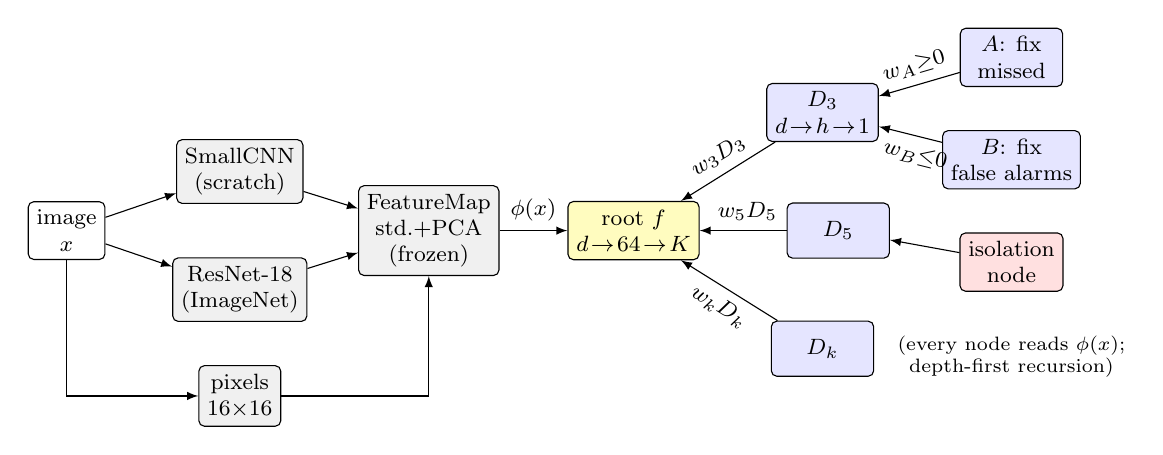
\begin{tikzpicture}[
  font=\footnotesize, >=latex,
  box/.style={draw, rounded corners=2pt, align=center, inner sep=3pt, minimum height=7mm},
  trunk/.style={box, fill=gray!12},
  node/.style={box, fill=blue!10, minimum width=13mm},
  root/.style={box, fill=yellow!25, minimum width=15mm},
  iso/.style={box, fill=red!12, minimum width=13mm},
]
\node[box, fill=white] (img) at (0,0) {image\\$x$};
\node[trunk] (t1) at (2.2,0.75) {SmallCNN\\(scratch)};
\node[trunk] (t2) at (2.2,-0.75) {ResNet-18\\(ImageNet)};
\node[trunk] (t0) at (2.2,-2.1) {pixels\\$16{\times}16$};
\node[trunk] (fm) at (4.6,0) {FeatureMap\\std.+PCA\\(frozen)};
\draw[->] (img) -- (t1); \draw[->] (img) -- (t2); \draw[->] (img) |- (t0);
\draw[->] (t1) -- (fm); \draw[->] (t2) -- (fm); \draw[->] (t0) -| (fm);
\node[root] (r) at (7.2,0) {root $f$\\$d\!\to\!64\!\to\!K$};
\draw[->] (fm) -- node[above]{$\phi(x)$} (r);
\node[node] (d1) at (9.6,1.5) {$D_3$\\$d\!\to\!h\!\to\!1$};
\node[node] (d2) at (9.8,0) {$D_5$};
\node[node] (d3) at (9.6,-1.5) {$D_k$};
\draw[->] (d1) -- node[above, sloped]{$w_3 D_3$} (r);
\draw[->] (d2) -- node[above, pos=0.45]{$w_5D_5$} (r);
\draw[->] (d3) -- node[below, sloped]{$w_k D_k$} (r);
\node[node] (a) at (12.0,2.2) {$A$: fix\\missed};
\node[node] (b) at (12.0,0.9) {$B$: fix\\false alarms};
\draw[->] (a) -- node[above, sloped]{$w_A{\ge}0$} (d1);
\draw[->] (b) -- node[below, sloped, pos=0.35]{$w_B{\le}0$} (d1);
\node[iso] (i1) at (12.0,-0.4) {isolation\\node};
\draw[->] (i1) -- (d2);
\node[font=\scriptsize, align=center] at (12.0,-1.6) {(every node reads $\phi(x)$;\\depth-first recursion)};
\end{tikzpicture}
\caption{Architecture. A frozen trunk and a frozen FeatureMap produce $\phi(x)$, which is shared by
every node. The $K$-way root is corrected by per-class detectors $D_k$ (our multiclass
generalisation of Table~II); every binary node is itself corrected by children $A$ (fires on its
misses) and $B$ (fires on its false alarms) exactly as in the note, recursively, with
closed-form isolation nodes as guaranteed-termination leaves. For Cats vs Dogs the root is a binary
node and the tree is the note's tree verbatim.}
\label{fig:arch}
\end{figure}

%% ---------------------------------------------------------------------------------------
\section{Providing features to the tree}
\label{sec:features}

A tree of small MLPs on raw $32{\times}32{\times}3$ or $64{\times}64{\times}3$ pixels can be grown to
100\% training accuracy, but every node then has to rediscover edges, colours and parts, and nodes
that only see pixels generalise poorly (\S\ref{sec:results}). We therefore separate
\emph{representation} from \emph{decision}: a frozen \emph{trunk} maps an image to a feature vector,
a fixed \emph{FeatureMap} standardises it and projects it onto its top principal components
(128 by default), and every node of the tree is a small network on this vector. Because the
FeatureMap is a fixed differentiable linear map, every node remains a differentiable function of the
\emph{image}, which is what we use to visualise receptive fields (\S\ref{sec:rf}).

We compare four ways of providing features (Fig.~\ref{fig:arch}):
\begin{enumerate}[leftmargin=*,itemsep=1pt]
\item \textbf{Pixels} -- no trunk; the image is area-downsampled to $16{\times}16$ (768-d) before PCA.
\item \textbf{Scratch CNN trunk} -- a 6-layer VGG-style CNN (32-64-128 channels, 0.29\,M parameters;
      stride-2 first layer for $64{\times}64$ inputs) trained from scratch on each dataset with
      crop/flip augmentation for 15 epochs, then frozen; 128-d global-average-pooled features.
\item \textbf{Transfer trunk} -- an ImageNet-1k ResNet-18 (\texttt{timm} \emph{a1} weights), frozen;
      images are resized to $128{\times}128$; 512-d pooled features. This trunk has never seen the
      target training set, so it cannot have memorised it.
\item \textbf{A set of trunks with per-node selection} -- both trunks are given their own FeatureMap, and
      \emph{every node trains one candidate network per trunk and keeps the one with the lowest
      training error}. This is node-level feature (block) selection, the note's open question 5.
\end{enumerate}
\textbf{A trap: features that have already memorised the data.} A trunk trained on the very samples
the tree must fit has partially memorised them; the tree then appears small and ``easy'' simply because
the overfitting happened in the trunk. To measure this we also trained the CNN trunk on a fixed half
$S_A$ of CIFAR-10 and grew one tree on $S_A$ and one on the unseen half $S_B$ (\S\ref{sec:results}).

%% ---------------------------------------------------------------------------------------
\section{Implementation}
\label{sec:impl}
The code (PyTorch, $\approx$2\,000 lines) is organised as a small library \texttt{treenn/} plus
experiment scripts; Table~\ref{tab:impl} lists the settings used throughout. All experiments ran on a
2-core CPU without a GPU, which is why the trunks are frozen and features are cached once: growing a
complete CIFAR-10 tree then takes 2--10 minutes.

\begin{table}[h]
\centering\small
\caption{Settings used for every tree unless stated otherwise.}
\label{tab:impl}
\begin{tabular}{@{}l>{\raggedright\arraybackslash}p{0.78\linewidth}@{}}
\toprule
Data & CIFAR-10: 50\,000 / 10\,000 ($32{\times}32$). Cats vs Dogs (Kaggle): 19\,989 / 5\,000, resized + centre-cropped to $64{\times}64$\\
FeatureMap & standardise $\to$ PCA (128 components, fit on the training set) $\to$ standardise\\
Root ($K$-way) & MLP $128\!\to\!64\!\to\!K$, cross-entropy, Adam (lr $10^{-2}$), 100 epochs, batch 8192\\
Binary nodes & MLP $128\!\to\!h\!\to\!1$ ($h=8$ unless stated; $h=0$: single neuron), weighted hinge \eqref{eq:node}, Adam (lr $10^{-2}$), up to 300 epochs, early stop as soon as the node makes zero errors\\
Connection weights & closed form \eqref{eq:closed}, $\delta=1$ (LP (6)--(9) via HiGHS when \texttt{--resolve lp})\\
Isolation fallback & child fixes none of its positives, or makes $>3\times$ the errors it was asked to fix, or depth $>10$\\
CNN trunk & 6 conv layers, SGD+Nesterov, one-cycle lr 0.05, wd $5\cdot10^{-4}$, batch 128, 15 epochs, crop+flip\\
\bottomrule
\end{tabular}
\end{table}

\noindent\textbf{Bookkeeping.} Every node stores the indices of the samples it was trained on and its
targets, so after training we can (i) check that the tree is exactly correct on every training
sample, (ii) attribute test-time changes of the prediction to individual children, (iii) prune nodes
while provably preserving training decisions (\S\ref{sec:min}), and (iv) visualise each node's
receptive field on the images it is responsible for (\S\ref{sec:rf}).

%% ---------------------------------------------------------------------------------------
\section{Results: overfitting to 100\% training accuracy}
\label{sec:results}

Table~\ref{tab:main} is the main result. Every configuration reaches \textbf{100.0\% training
accuracy}; we verify this on every training sample after the tree is built, not from the training
loss. The columns ``root'' give the accuracy of the root network alone (what an ordinary small
network achieves), ``nodes (isol.)'' counts all networks in the tree, root included, and how many of
them are closed-form isolation nodes, and ``test fixed/broken'' attributes every test prediction that the
children changed: \emph{fixed} if the root was wrong and the tree is right, \emph{broken} if the root
was right and the tree is wrong.

\begin{table}[t]
\centering\small
\caption{Trees grown to 100\% training accuracy. Root = the root network alone. ``Test fixed/broken''
counts test images whose prediction the children changed from wrong to right / right to wrong.}
\label{tab:main}
\resizebox{\linewidth}{!}{\begin{tabular}{@{}lrrrrrrrr@{}}\toprule
 & \multicolumn{2}{c}{root acc. (\%)} & \multicolumn{2}{c}{tree acc. (\%)} & nodes & & & test fixed/\\
\cmidrule(lr){2-3}\cmidrule(lr){4-5}
configuration & train & test & train & test & (isol.) & params & depth & broken\\\midrule
\multicolumn{9}{@{}l}{\emph{CIFAR-10 -- corrector tree, root $128\to64\to10$, binary nodes $h=8$}}\\
pixels & 60.6 & 50.8 & 100.0 & \textbf{48.5} & 107 (6) & 1470.1k & 10 & 395/627\\
scratch CNN & 92.1 & 84.8 & 100.0 & \textbf{81.8} & 83 (2) & 144.0k & 6 & 109/406\\
ResNet-18 (ImageNet) & 84.2 & 74.5 & 100.0 & \textbf{69.8} & 67 (0) & 77.6k & 4 & 256/729\\
CNN + ResNet, per-node trunk selection & 92.1 & 84.8 & 100.0 & \textbf{82.2} & 35 (0) & 44.3k & 4 & 167/422\\
\midrule
\multicolumn{9}{@{}l}{\emph{Cats vs Dogs -- the note's binary tree, every node $128\to h\to1$}}\\
pixels & 71.5 & 63.2 & 100.0 & \textbf{59.8} & 38 (0) & 39.6k & 6 & 439/606\\
scratch CNN & 96.1 & 94.1 & 100.0 & \textbf{92.1} & 17 (1) & 17.4k & 4 & 54/155\\
ResNet-18 (ImageNet) & 97.9 & 93.4 & 100.0 & \textbf{93.2} & 5 (0) & 5.2k & 2 & 40/50\\
CNN + ResNet, per-node trunk selection & 97.9 & 93.4 & 100.0 & \textbf{93.3} & 5 (0) & 5.2k & 2 & 40/45\\
scratch CNN, single neurons ($h=0$, the note) & 95.8 & 93.6 & 100.0 & \textbf{93.6} & 3 (2) & 107.7k & 1 & 1/1\\
scratch CNN, $h=8$, LP (6)--(9) + $\ell_1$ & 96.2 & 94.0 & 100.0 & \textbf{92.1} & 17 (1) & 17.4k & 4 & 50/145\\
\bottomrule\end{tabular}
}
\end{table}

\begin{figure}[t]
\centering
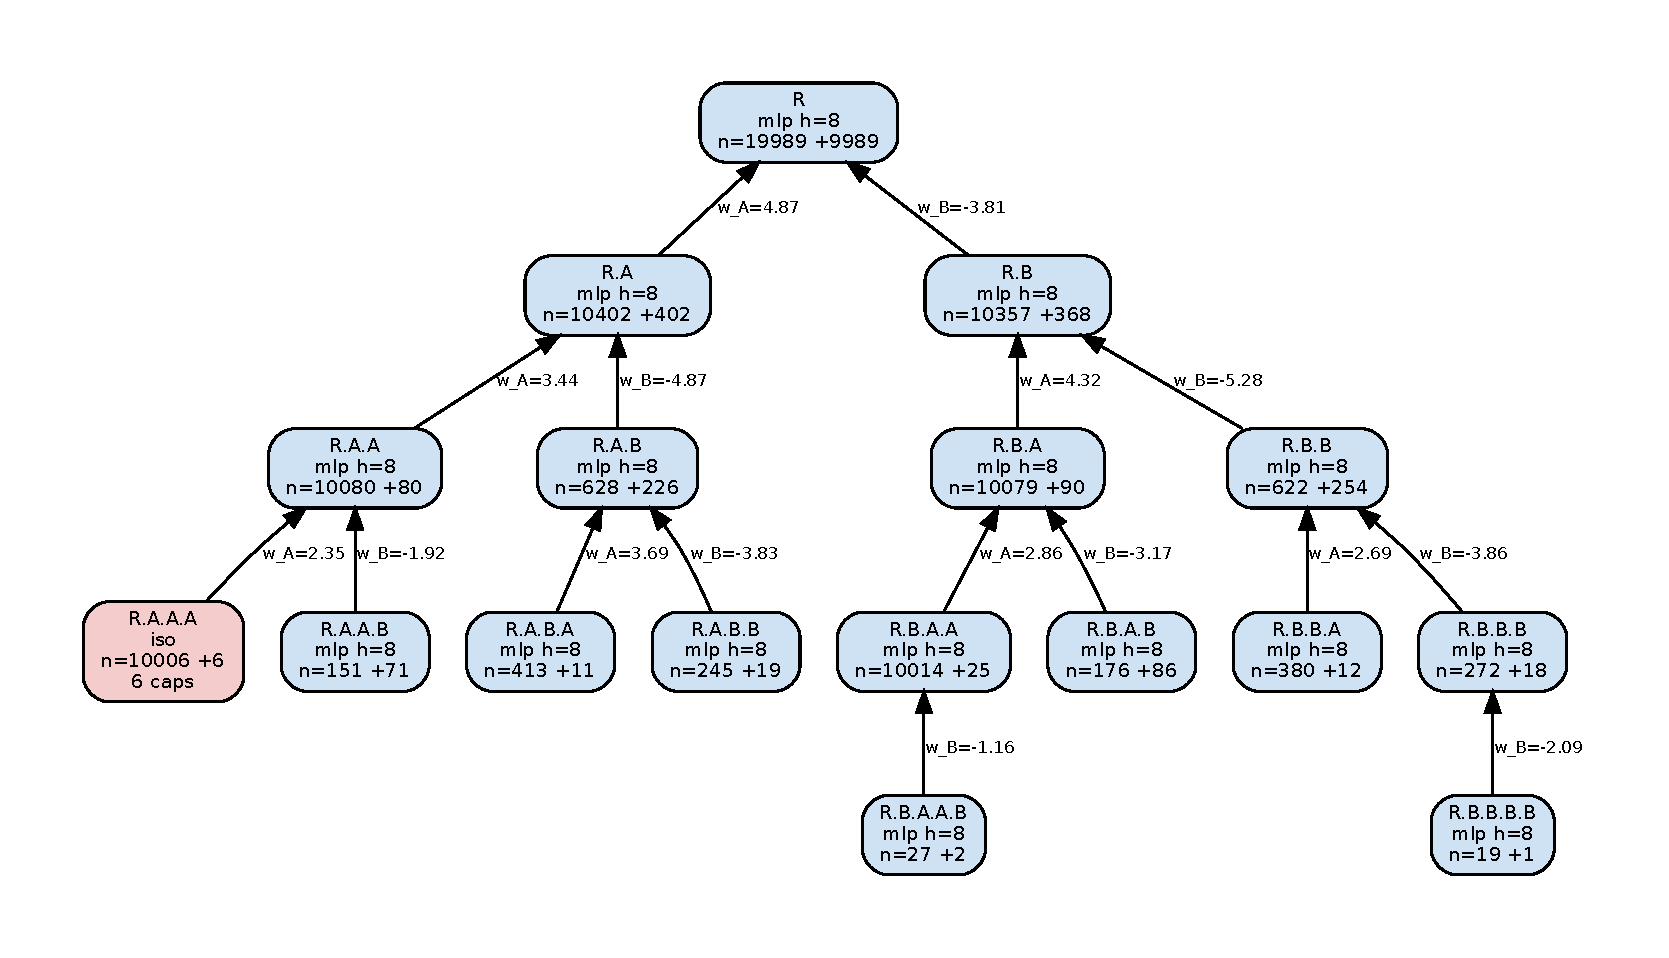
\includegraphics[width=\linewidth]{tree_cd_cnn.pdf}
\caption{The Cats vs Dogs tree (CNN trunk, $h=8$), drawn like Fig.~4 of the note: each box is a
$128\!\to\!8\!\to\!1$ network trained on $n$ samples of which ``$+m$'' must make it fire; arrows carry
the closed-form connection weights \eqref{eq:closed}. A is always the ``missed'' child and B the
``false-alarm'' child. One child (red) could not make progress and became an isolation node with 6
caps. The tree classifies all 19\,989 training images correctly.}
\label{fig:treecd}
\end{figure}

\paragraph{Overfitting is always achieved, at very different costs.}
As with deep networks trained on random labels~\cite{zhang},
reaching 100\% is never the hard part. How many nodes interpolation needs is set by how far the root is from interpolating, i.e.\ by the
features. On Cats vs Dogs the ImageNet trunk leaves the root at 97.9\% training accuracy and the whole
tree has five nodes; with the scratch CNN it has 17, with pixels 38. On CIFAR-10 the root leaves 7.9k
(ResNet), 3.9k (CNN) or 19.7k (pixel) training errors and the corrector tree grows to
67, 83 and 107 nodes (the pixel tree reaches the depth limit and needs 1.47M parameters). In the paper's own setting -- every node a \emph{single} neuron
($h=0$) on CNN features -- the root neuron already reaches 95.8\%/93.6\%, but neither linear child
can solve its sub-problem: the balanced linear child $A$ catches 384 of the 404 missed dogs at the
price of 2\,076 false alarms. These ``inside-out'' sub-problems (positives surrounded by the
parent's correctly classified negatives) are exactly what made the MNIST tree of the first assignment
deep; here both children fall back to isolation nodes. With $h=8$ hidden units all but one child make
progress and the tree reaches depth 4 with a single isolation leaf.

\paragraph{The LP (6)--(9) and the redundant slacks.} Re-solving each node's output layer
together with $(w_A,w_B)$ as the note's LP (HiGHS, $\ell_1$ weight $10^{-3}$) gives \emph{exactly zero
total slack at every one of the 9 internal nodes} of the Cats vs Dogs tree -- the slacks are redundant,
as the note says -- and the same tree to within 0.06\% test accuracy (92.12\% vs 92.06\%). The LP
solutions are vertices with large connection weights ($w_A=232$, $w_B=-169$ at the root, versus
4.9 and $-3.8$ in closed form \eqref{eq:closed}), the badly scaled regime in which an LP solver can
report spurious non-zero slacks.

\paragraph{Interpolation lowers test accuracy, because the correctors generalise.}
Whenever the children are learned networks, the tree is \emph{worse} on test data than its own
root (by 0.1--4.7 points; Table~\ref{tab:main}), and the fixed/broken column shows why: each child is a small network trained on its
own few hundred or thousand positives, it learns a decision region rather than a list of points, and
on test images that region also covers images the root had right. Corrections break 1.3--4.4 test
predictions for every one they fix. This is the classical over-fitting picture, made visible node
by node.

\begin{table}[t]
\centering\small
\caption{Width of the binary nodes (CIFAR-10, ResNet trunk, corrector tree; root fixed at
$128\!\to\!64\!\to\!10$, 84.2\% train / 74.5\% test). ``Isolation only'' replaces every child by a
closed-form isolation node.}
\label{tab:width}
\resizebox{\linewidth}{!}{\begin{tabular}{@{}lrrrrrrrr@{}}\toprule
 & \multicolumn{2}{c}{root acc. (\%)} & \multicolumn{2}{c}{tree acc. (\%)} & nodes & & & test fixed/\\
\cmidrule(lr){2-3}\cmidrule(lr){4-5}
configuration & train & test & train & test & (isol.) & params & depth & broken\\\midrule
$h=0$ (linear $\to$ all isolation) & 84.2 & 74.5 & 100.0 & \textbf{74.6} & 11 (10) & 1027.5k & 1 & 10/0\\
$h=2$ & 84.2 & 74.5 & 100.0 & \textbf{73.3} & 93 (13) & 842.2k & 8 & 101/224\\
$h=8$ & 84.2 & 74.5 & 100.0 & \textbf{69.8} & 67 (0) & 77.6k & 4 & 256/729\\
$h=32$ & 84.2 & 74.5 & 100.0 & \textbf{70.7} & 18 (0) & 79.6k & 2 & 277/653\\
$h=128$ & 84.2 & 74.5 & 100.0 & \textbf{72.6} & 16 (0) & 258.5k & 2 & 284/475\\
isolation nodes only & 84.2 & 74.5 & 100.0 & \textbf{74.6} & 11 (10) & 1027.5k & 1 & 10/0\\
\bottomrule\end{tabular}
}
\end{table}

\paragraph{Benign versus harmful interpolation.} Table~\ref{tab:width} varies the width of the
correcting networks with the root held fixed. Linear children ($h=0$) never make progress, so the
tree consists of the root plus ten isolation nodes with 7\,902 caps -- one per training error -- and
its test accuracy is the root's: the caps changed only 10 of 10\,000 test predictions, all ten for
the better. The same holds when isolation is forced. Learned correctors are 13$\times$ smaller
(77.6k vs 1.03M parameters) but cost 1.2--4.7 points; the damage is largest for $h=8$--32 and
shrinks again for $h=128$, whose wider detectors fit their positives with tighter regions. This is
the sharpest form of the trade-off behind the whole assignment: \emph{memorising like a lookup table is
harmless but large; memorising with a small network is compact but generalises the noise.}

\begin{table}[t]
\centering\small
\caption{Multiclass extensions (CIFAR-10, ResNet trunk, $h=8$).}
\label{tab:archs}
\resizebox{\linewidth}{!}{\begin{tabular}{@{}lrrrrrrrr@{}}\toprule
 & \multicolumn{2}{c}{root acc. (\%)} & \multicolumn{2}{c}{tree acc. (\%)} & nodes & & & test fixed/\\
\cmidrule(lr){2-3}\cmidrule(lr){4-5}
configuration & train & test & train & test & (isol.) & params & depth & broken\\\midrule
one-vs-rest forest & 83.2 & 75.0 & 100.0 & \textbf{67.1} & 145 (0) & 150.9k & 5 & 467/1252\\
corrector tree & 84.2 & 74.5 & 100.0 & \textbf{69.8} & 67 (0) & 77.6k & 4 & 256/729\\
gated tree & 84.2 & 74.5 & 100.0 & \textbf{73.6} & 13 (1) & 918.3k & 5 & 27/118\\
\bottomrule\end{tabular}
}
\end{table}

\paragraph{Multiclass architectures (Table~\ref{tab:archs}).} The one-vs-rest forest is the most
expensive and the worst: ten independent roots make 10$\times$ more decisions, each binary root
errs on its own samples, and the forest needs 145 nodes and 151k parameters (67.1\% test). The
corrector tree shares one $K$-way root and grows detectors only for classes with errors (67 nodes,
77.6k). The gated tree is the most instructive: its re-classifier $R$ is easy (it relearns the 7\,902
errors of the root with only 31 mistakes), but its error detector $E$ must answer ``is the root wrong
here?'', which is as hard as the original problem -- the $h=8$ detector finds only 1\,060 of the 7\,902
errors and its missed-error child falls back to a 6\,839-cap isolation node. Detecting one's own errors
does not get easier by moving it into a separate node.

\begin{table}[t]
\centering\small
\caption{A trunk that has seen the data hides overfitting. CNN trunk trained on half $S_A$ of
CIFAR-10 (82.5\% test); trees grown on $S_A$ and on the unseen half $S_B$ (25k images each).}
\label{tab:half}
\resizebox{\linewidth}{!}{\begin{tabular}{@{}lrrrrrrrr@{}}\toprule
 & \multicolumn{2}{c}{root acc. (\%)} & \multicolumn{2}{c}{tree acc. (\%)} & nodes & & & test fixed/\\
\cmidrule(lr){2-3}\cmidrule(lr){4-5}
configuration & train & test & train & test & (isol.) & params & depth & broken\\\midrule
tree on $S_A$ (trunk's own training half) & 90.2 & 81.2 & 100.0 & \textbf{78.5} & 61 (0) & 71.4k & 6 & 149/427\\
tree on $S_B$ (half never seen by the trunk) & 85.0 & 81.7 & 100.0 & \textbf{76.3} & 95 (2) & 104.9k & 7 & 218/756\\
\bottomrule\end{tabular}
}
\end{table}

\paragraph{Where the memorisation lives (Table~\ref{tab:half}).} With features from a trunk that was
trained on $S_A$, the root fits $S_A$ to 90.2\% but the unseen $S_B$ only to 85.0\%, while both roots
test at $\approx$81.5\%. The 5-point gap is memorisation that already happened inside the trunk, and
the tree pays for it on $S_B$: 95 instead of 61 nodes and 47\% more parameters. When features come from
a trunk trained on the same images, a small tree is therefore \emph{not} evidence of an easy problem.
This is why the ImageNet trunk, which never saw the target images, is the cleanest place to study
interpolation in the tree itself, and why we use it for the double-descent experiments.

\paragraph{A set of trunks, chosen per node.} When every node may choose between the CNN and the
ResNet features (Table~\ref{tab:main}), the roots choose the trunk with the lower training error
(CNN on CIFAR-10, ResNet on Cats vs Dogs) but \emph{all ten} first-level detectors on CIFAR-10 choose the
ResNet features, and deeper nodes alternate (depth 2: 7 CNN / 7 ResNet; depth 3: 6/2). The root's
errors are exactly the images on which the CNN's features are ambiguous, so they are best separated in
a different feature space. The resulting tree is 2.4$\times$ smaller than the CNN-only tree (35 vs 83
nodes, 44k vs 144k parameters) and better on test data (82.2\% vs 81.8\%).

%% ---------------------------------------------------------------------------------------
\section{Double descent}
\label{sec:dd}

\paragraph{Protocol.} Double descent is easiest to see with few samples and label noise
\cite{belkin,nakkiran}, so we use $n=4\,000$ CIFAR-10 training images (ImageNet trunk, PCA-64), with
clean labels and with 20\% of the labels replaced by a random wrong class, and the full 10\,000-image
test set. For every width $H\in\{1,2,4,\dots\}$ we train one MLP $64\!\to\!H\!\to\!10$ with
full-batch Adam for 3\,000 steps and no regularisation, and then grow a corrector tree that uses
\emph{that same MLP as its root} and binary nodes of width $H$, until it interpolates. The two curves in
Fig.~\ref{fig:dd} therefore differ only by the children.

\begin{figure}[t]
\centering
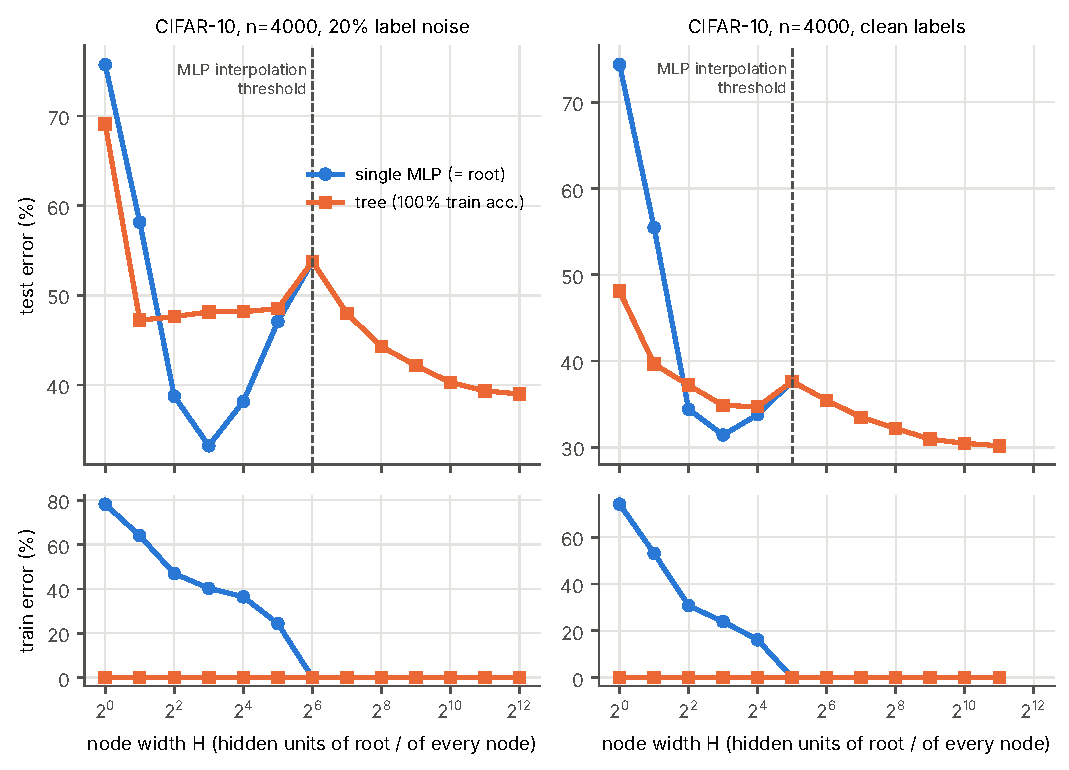
\includegraphics[width=0.8\linewidth]{double_descent.pdf}
\caption{Model-wise double descent on CIFAR-10 ($n=4\,000$). Blue: the root MLP alone; orange: the
tree built on that root, which always reaches 0\% training error. Dashed line: the smallest width at
which the MLP itself interpolates.}
\label{fig:dd}
\end{figure}

\paragraph{The root network shows a textbook double descent.} With 20\% noise (Fig.~\ref{fig:dd},
left) the MLP's test error falls from 75.7\% ($H=1$) to 33.2\% ($H=8$), the classical sweet spot, then
\emph{rises} to 53.8\% at $H=64$ -- precisely the first width whose training error is zero, where it has
memorised all 815 corrupted labels -- and then falls again monotonically to 39.0\% at $H=4\,096$
(307k parameters, $7.7\times$ more than $nK=40$k). The test cross-entropy peaks at the same width
(7.7 vs 1.06 at $H=8$). With clean labels (right) the curve has the same shape but a smaller peak at a
smaller width: 31.4\% at $H=8$, 37.7\% at the first interpolating width $H=32$, and 30.2\% at
$H=2048$ -- here the over-parameterised branch ends \emph{below} the classical optimum. Noise moves the
interpolation threshold to the right (noisy labels need more capacity to memorise) and makes the
peak higher (memorising them at the threshold forces the least smooth interpolant).

\paragraph{The tree never sees the classical regime.} For $H$ at or above the threshold the root
interpolates on its own, no children are grown, and the two curves coincide -- including the peak,
so the tree's own error-versus-width curve has the double-descent shape too, with its peak at the
width at which the \emph{root} can just interpolate. Below the threshold the children force
interpolation and the tree's error is almost flat (noisy: 47.2--48.5\% for $H=2$--32; clean:
34.7--39.7\% for $H=2$--16), close to the error of the MLP just past its peak. Growing children is a
second way to cross the interpolation threshold: instead of widening one network we add small ones
until the data are memorised. Fig.~\ref{fig:ddp} places the trees on the parameter axis: for $H\ge2$ they hold 12k--95k
parameters, one to two orders of magnitude more than their roots and as many as MLPs of width $H=256$--1024, and their
test error is within a few points of those MLPs on the over-parameterised branch (noisy: 47--48\% vs
40--44\%) -- not that of the small root they started from (33\% at $H=8$).

\begin{figure}[t]
\centering
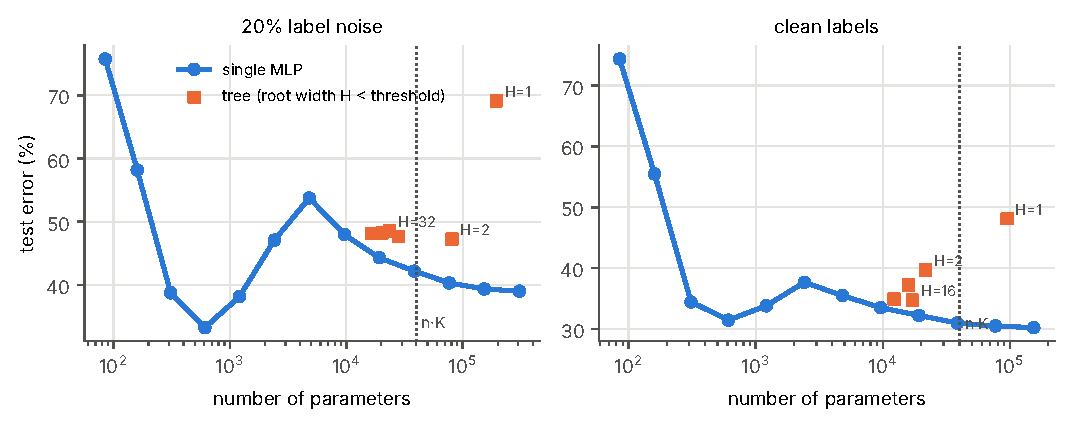
\includegraphics[width=0.8\linewidth]{double_descent_params.pdf}
\caption{The same runs against the number of parameters (log scale). Trees (squares, root width
$H$ below the threshold) sit with the over-parameterised MLPs, not with their own small roots.}
\label{fig:ddp}
\end{figure}

\paragraph{Children help an under-fitted root and hurt a well-fitted one.} At $H=1$--2 the root is
far from the data and the children act as a boosting stage: with clean labels the tree on a
width-1 root has 48.1\% error instead of 74.4\% (2\,916 test predictions fixed, 290 broken). From
$H=4$ on, the root is close to its best test error and the children mostly memorise its residual --
with noise, mostly the corrupted labels -- and break more than they fix (e.g.\ $H=8$, noisy: 296
fixed, 1\,788 broken). Every tree memorises 100\% of the corrupted labels; the roots below the threshold memorise
4--11\% of them ($H\le16$), rising to 39\% at $H=32$.

\paragraph{Where does the label noise go?} We grew a tree on 10\,000 CIFAR-10 images with 20\%
corrupted labels (ResNet trunk, $h=8$; 25 nodes, 100\% training accuracy, test accuracy 56.1\%$\to$50.7\%).
Fig.~\ref{fig:noise} follows the corrupted labels through it. The root memorises 47\% of them by
itself, but its training errors are 55\% corrupted labels against 20\% in the data -- the root learns
the clean structure and leaves most of the noise to its children, whose first level is therefore
mostly a \emph{noise memoriser}. Deeper nodes, which correct the detectors' own false alarms and
misses, receive clean labels again (22\% at depth 2, none at depth 3). In this sense a tree separates
signal (root) from memorisation (children) by construction, and \S\ref{sec:min} shows that removing
children is the simplest way to recover the root's generalisation.

\begin{figure}[h]
\centering
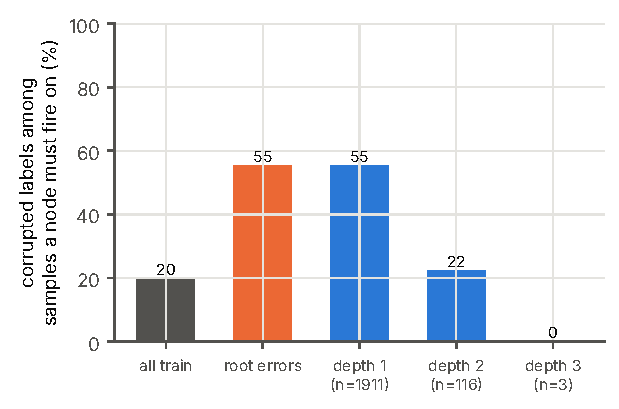
\includegraphics[width=0.5\linewidth]{noise_depth.pdf}
\caption{Fraction of corrupted labels among the samples that each part of the tree must fire on
(CIFAR-10, 10k images, 20\% symmetric noise).}
\label{fig:noise}
\end{figure}

%% ---------------------------------------------------------------------------------------
\section{Receptive fields of nodes}
\label{sec:rf}

Since trunk, FeatureMap and node are all differentiable, the receptive field of node $v$ can be
read off in image space. For each node we show (i) the six training images on which the node's own
network $f_v$ responds most strongly (among the samples the node was trained on), (ii) the saliency
$|\partial f_v/\partial x|$ of the top image~\cite{simonyan}, and (iii) the mean saliency map over up
to 32 of the node's positives. We quantify the maps by the \emph{area-50} (the fraction of pixels
needed to hold 50\% of the saliency mass; 0.5 would be uniform) and the \emph{centre mass} (saliency
inside the central quarter of the image; 0.25 would be uniform).

\begin{figure}[p]
\centering
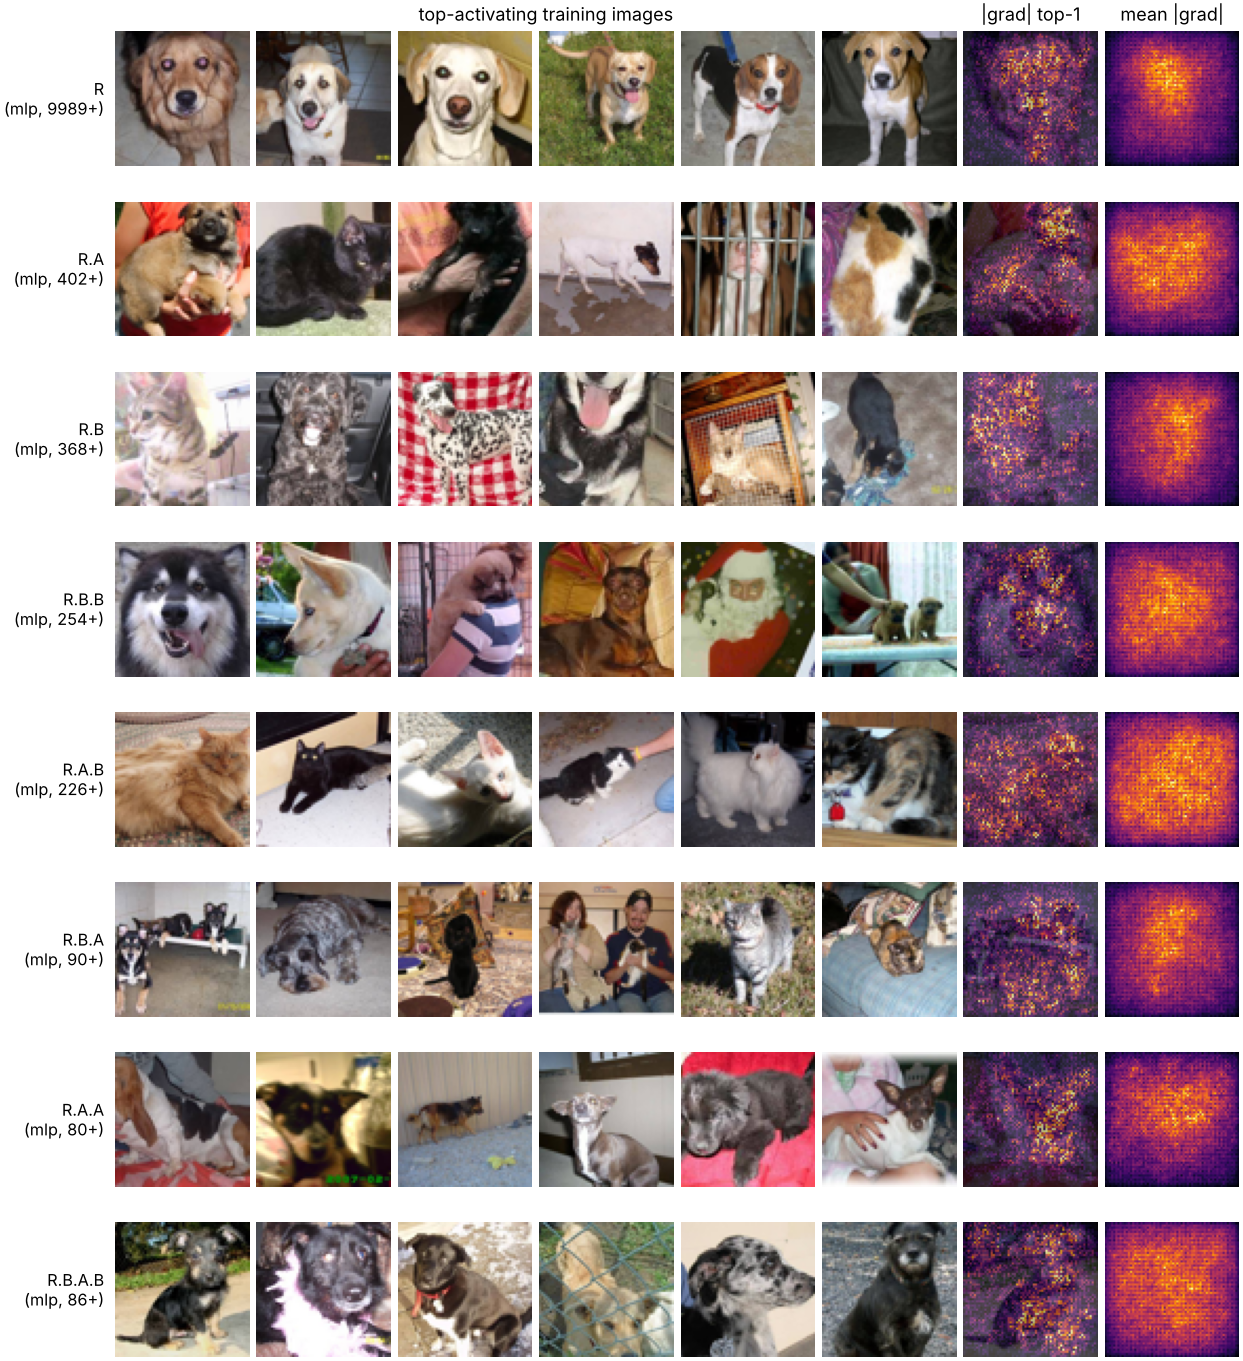
\includegraphics[width=0.74\linewidth]{rf_catsdogs_cnn_binary_h8_n0.0_nodes0.png}\\[2pt]
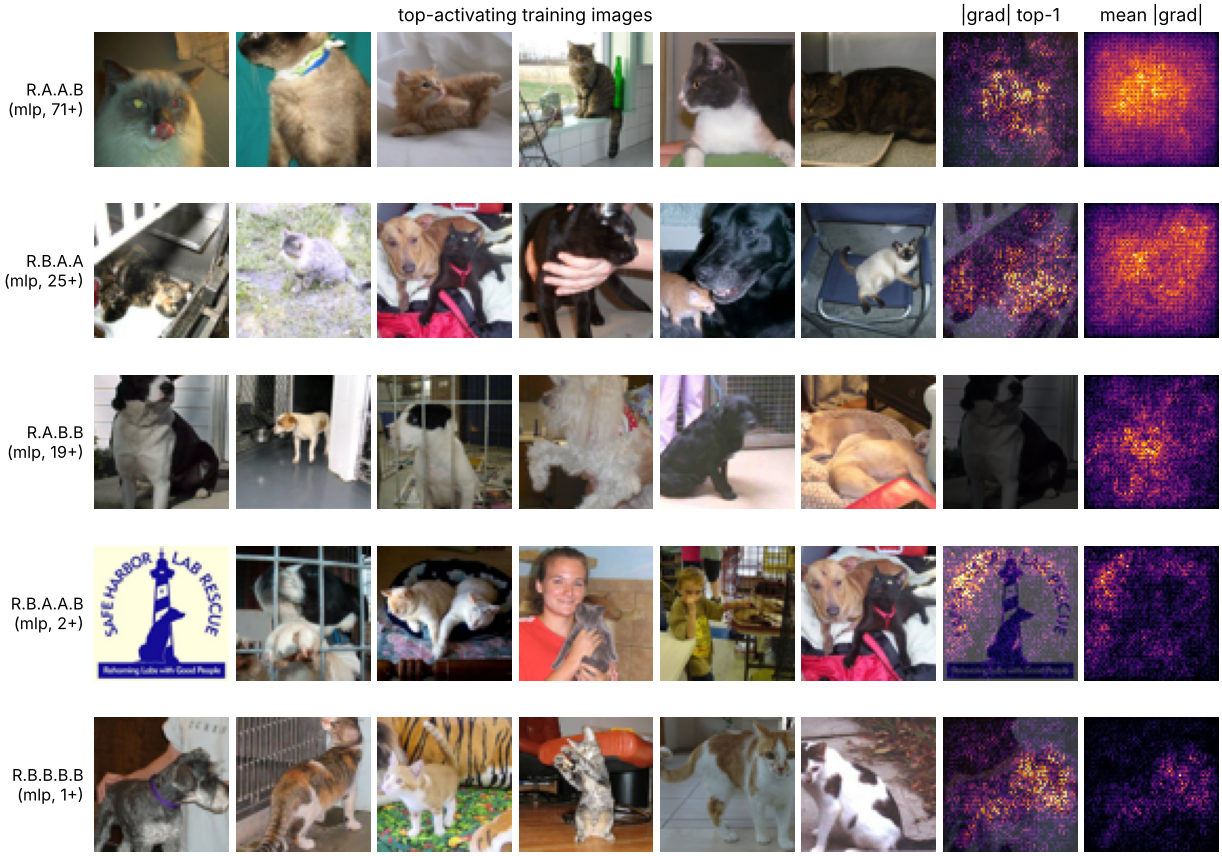
\includegraphics[width=0.74\linewidth]{rf_catsdogs_cnn_binary_h8_n0.0_nodes1.png}
\caption{Receptive fields of the Cats vs Dogs tree of Fig.~\ref{fig:treecd} (CNN trunk). Rows are
nodes (path, kind, number of positives), ordered by depth; R fires for ``dog'', R.A fixes missed dogs,
R.B fixes cats taken for dogs, and so on. Columns: the six training images with the largest response
of the node's own network, the saliency of the top image (overlay), and the mean saliency over the
node's positives. Note R.B.A.A.B, a node with two positives whose top image is a rescue-centre logo
filed under ``dog''.}
\label{fig:rfcd}
\end{figure}

\begin{figure}[p]
\centering
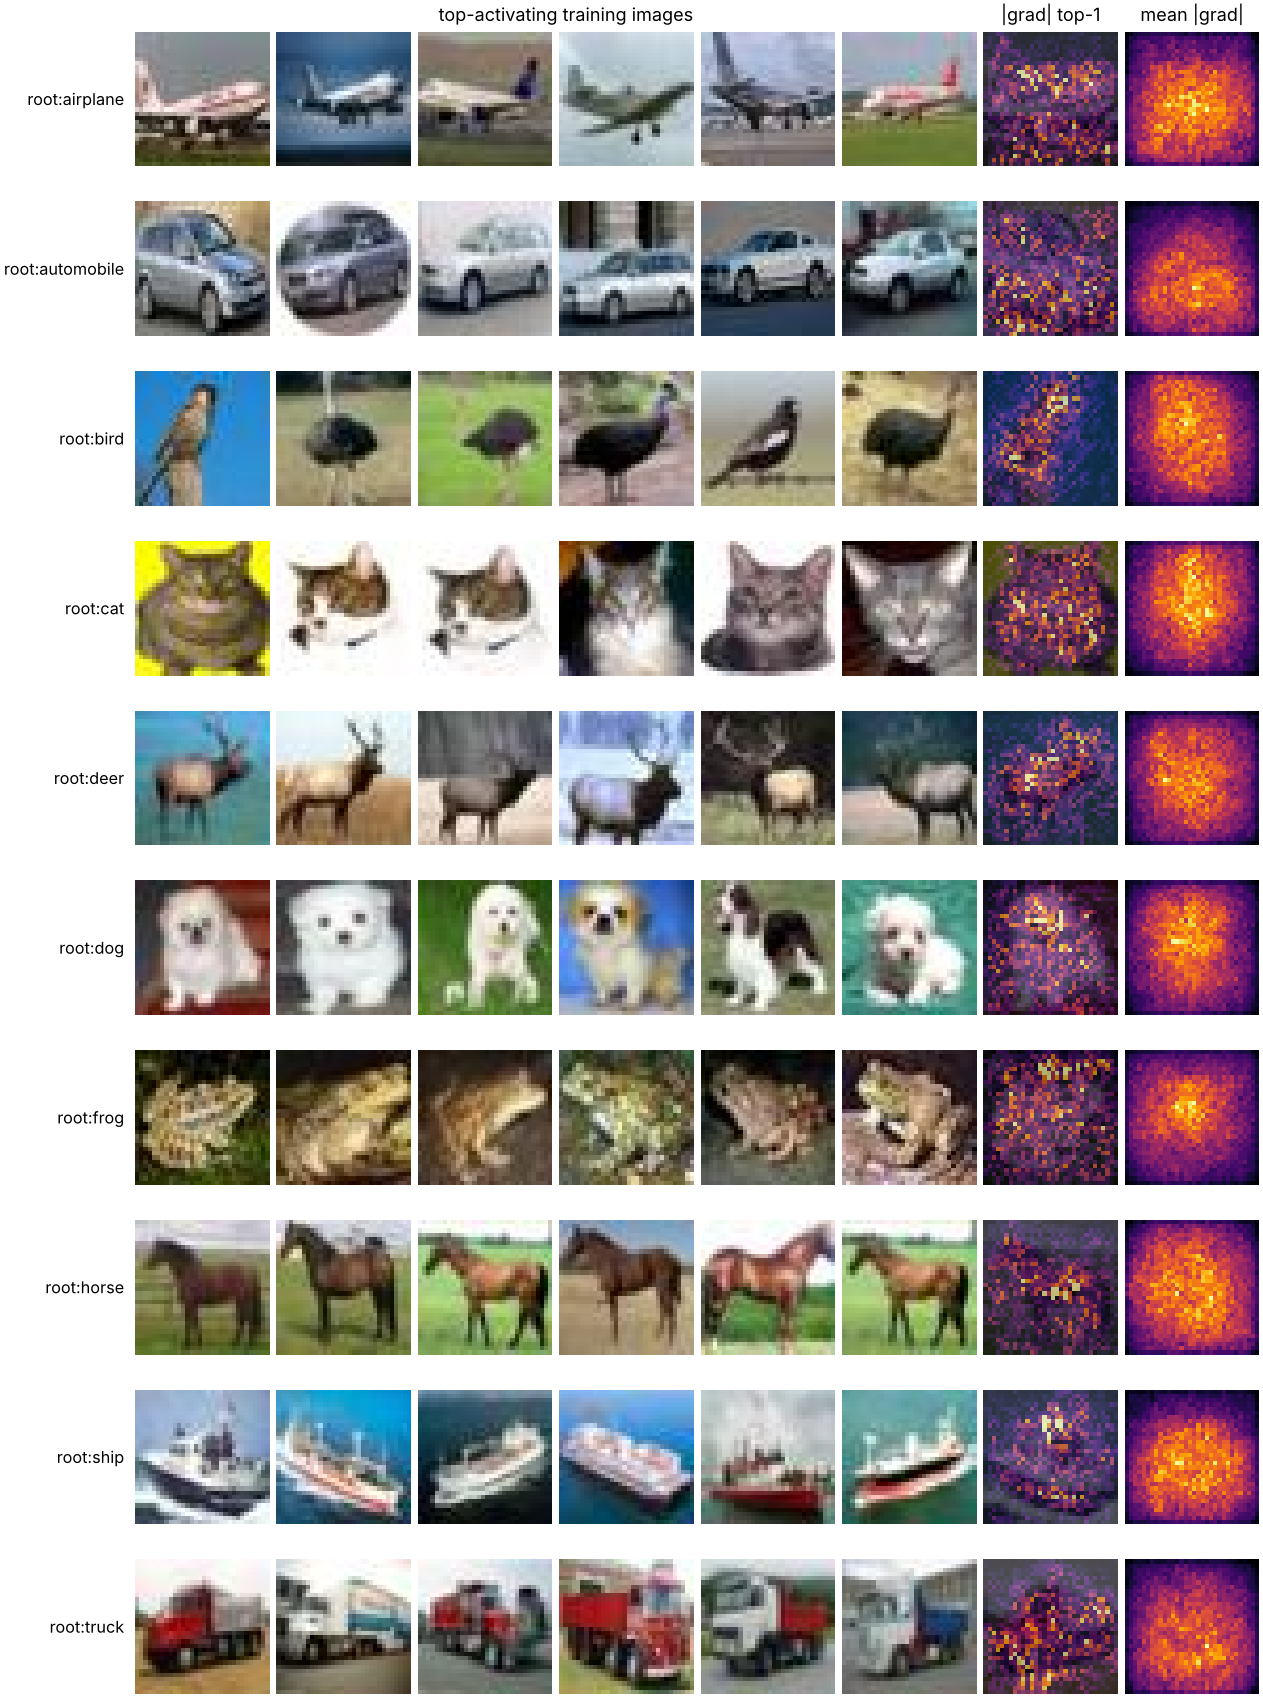
\includegraphics[width=0.85\linewidth]{rf_cifar10_cnn_corrector_h8_n0.0_root.png}
\caption{Per-class receptive fields of the CIFAR-10 root (CNN trunk): the class logit's top
training images, the saliency of the top image, and the mean saliency over correctly classified images
of that class.}
\label{fig:rfroot}
\end{figure}

\begin{figure}[t]
\centering
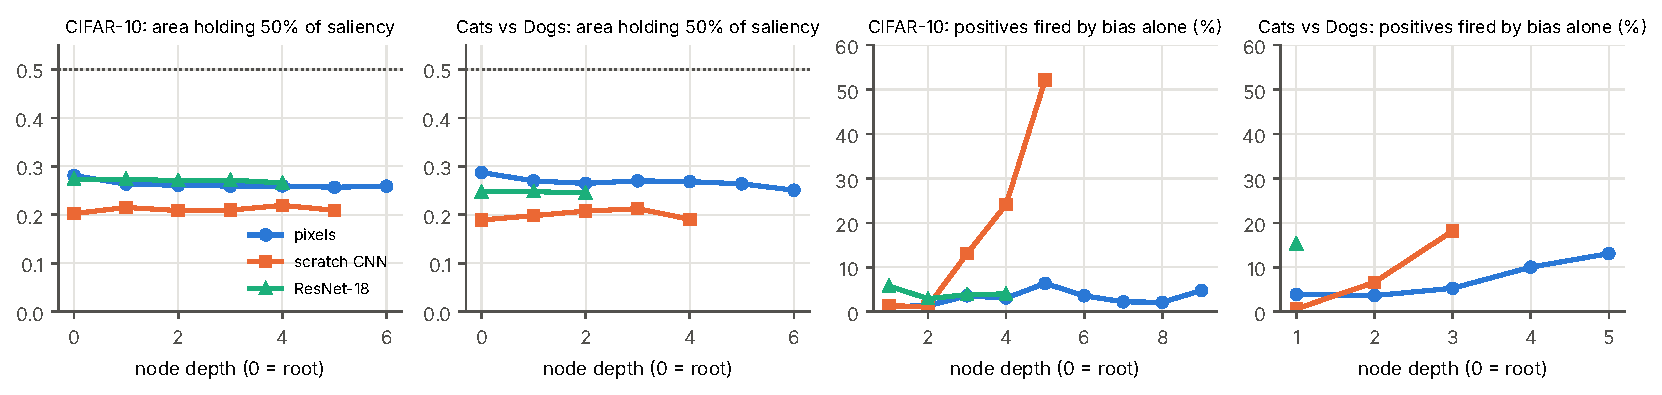
\includegraphics[width=\linewidth]{rf_depth.pdf}
\caption{Receptive-field statistics against depth. Left: area-50 of the saliency (largest four nodes
per depth; dotted: uniform map); it is set by the trunk, not by depth. Right: fraction of each depth's
positives on which every hidden unit of the node is silent, so that the node fires by its output bias
alone (all nodes; depths with fewer than 10 positives omitted).}
\label{fig:rfdepth}
\end{figure}

\paragraph{Roots are object-centred class templates.} The root's top images are canonical, centred
exemplars -- frontal dog faces on Cats vs Dogs (Fig.~\ref{fig:rfcd}, row R); side-on cars, trucks
and ships and close-up cat faces on CIFAR-10 (Fig.~\ref{fig:rfroot}) -- and its saliency is a compact
blob in the middle of the image (Cats vs Dogs, CNN trunk: half of the saliency lies in 19\% of the
pixels, and 38\% of it in the central quarter). With the
scratch CNN the saliency of every class is a centred disc; with the ImageNet trunk it is broader and
shows the bilinear up-sampling grid of the $32\to128$ resize, a reminder that a transferred trunk
looks at the image at a scale it was not trained for.

\paragraph{First-level children respond to atypical members of a class.} R.A (missed dogs) responds
to dogs that look unlike the root's template: puppies held in someone's arms, dark-coated dogs,
dogs behind bars. R.B (cats taken for dogs) responds to images whose context says ``dog'' -- a
dalmatian on a chequered cloth, a long-haired black-and-white animal -- i.e.\ these nodes encode
\emph{exceptions} to the root's rule, as the note's construction intends.

\paragraph{Deep nodes memorise idiosyncratic photographs.} Two or three levels further down, the
top images are cluttered, multi-object, or barely about the class at all: people holding cats, a dog
and a cat on one sofa, a Santa Claus picture (R.B.B), and at R.B.A.A.B a rescue-centre logo that the
dataset files under ``dog''. These are the long tail and the label errors of the dataset, and the tree
isolates them in its deepest nodes.

\paragraph{The trunk, not the depth, sets the spatial extent.} Perhaps surprisingly, the saliency of
deep nodes is \emph{not} more diffuse than the root's (Fig.~\ref{fig:rfdepth}, left): with the CNN trunk
half of the saliency lies in 19--22\% of the pixels at every depth, with the ResNet trunk in 25--28\%,
with pixels in 25--29\%. (Our first analysis suggested widening fields; it was an artefact of images on
which a node's gradient is exactly zero, which we now exclude -- and which turned out to be the real
story, below.) With pixel features even the root is not object-centred (Cats vs Dogs: 24\% of the
saliency in the central quarter, i.e.\ uniform, against 38\% with the CNN trunk): every pixel node keys on
global colour layout, which is why pixel trees generalise poorly.

\paragraph{Deep nodes recognise their positives by exclusion.} What does change with depth is
\emph{how} a node recognises its positives (Fig.~\ref{fig:rfdepth}, right). For a growing fraction of
a deep node's positives \emph{all} of its hidden units are silent, so the node fires on them purely
through a positive output bias, while almost none of its negatives ($\le$2\%) are in that state. With
the CNN trunk on CIFAR-10 this fraction rises from 1\% of the positives at depths 1--2 to 13\%, 24\% and
52\% at depths 3, 4 and 5 (Cats vs Dogs: 0.6\%$\to$7\%$\to$18\%). Such a node's hidden units are
\emph{veto} detectors that tile its negatives -- in R.A.A, 6 of 8 output weights are negative and the
output bias is $+0.92$ -- and the positives are simply ``whatever no veto recognises''. On these images
the input gradient is exactly zero: the node has no receptive field for what it detects, only for what
it rejects. A ``fire unless vetoed'' rule is the natural way for a small network to single out a few
points among thousands, and it generalises badly by design: any test image unlike all of the node's
training negatives triggers it.

\paragraph{Learned correctors over-generalise; isolation nodes do not.} The receptive fields explain
the fixed/broken column of \S\ref{sec:results} quantitatively. By construction, every CIFAR-10 detector
$D_k$ fires on \emph{none} of the training images of other classes, yet it fires on 1.9\% (ResNet) /
0.9\% (CNN) of the \emph{test} images of other classes -- each firing a candidate ``broken''
prediction -- while catching only 12\% / 8\% of the root's test errors on its own class. The
isolation-node detectors fire on 0.00\% of other-class test images and catch 0.4\% of the errors:
useless, but harmless.

%% ---------------------------------------------------------------------------------------
\section{Minimising the size of the network}
\label{sec:min}

``Size'' can be minimised at four levels; we tried all four and report parameters (or non-zero
weights) of everything below the trunk.

\paragraph{1. Design choices that shrink the tree at equal (100\%) training accuracy.}
(a) \emph{Node width} has an interior optimum (Table~\ref{tab:width}): linear or width-2 children
make no progress and fall back to isolation nodes that need one 129-parameter cap per memorised
image (0.84--1.03M parameters), very wide children are expensive per node (259k at $h=128$), and
$h=8$--32 gives the smallest trees (78--80k). (b) \emph{Sharing the root} across classes: the corrector
tree needs half the parameters of the one-vs-rest forest (Table~\ref{tab:archs}). (c) \emph{Letting
each node choose its trunk} gives the largest reduction we found: 144k$\to$44k parameters
(83$\to$35 nodes) on CIFAR-10 at higher test accuracy (Table~\ref{tab:main}).

\paragraph{2. Decision-preserving pruning.} For every node we search the highest sparsity
$s$ among 0.5, 0.8, 0.9, 0.95, 0.98 and 0.99 at which magnitude pruning~\cite{lottery} followed by a short masked
fine-tune leaves the node's decision on \emph{every one of its training samples} unchanged.
Because a node's decisions define its children's training sets (Table~II), this preserves the whole
tree's 100\% training accuracy by construction; only the connection weights are recomputed with
\eqref{eq:closed}. Table~\ref{tab:prune} shows 20--32\% fewer non-zero weights at unchanged training
accuracy and test accuracy within $\pm0.1$ points. The prunability is very uneven: nodes that serve a
few hundred samples prune to 80--95\% sparsity, while the root and the first-level detectors (which
must keep 45--50k decisions exactly) cannot be pruned even to 50\%. Pruning also performs the note's
\emph{feature selection} (open question 5): the sparsest nodes read only 34--40 of the 128 PCA features.

\begin{table}[h]
\centering\small
\caption{Decision-preserving pruning: every node keeps every training decision, so the tree stays at
100\% training accuracy.}
\label{tab:prune}
\resizebox{\linewidth}{!}{\begin{tabular}{@{}lrrrrrr@{}}\toprule
tree & non-zero weights & after pruning & reduction & train acc. & test acc. before & after\\\midrule
CIFAR-10, ResNet, corrector $h$=8 & 77\,612 & 58\,422 & 25\% & 100.0\% & 69.78\% & 69.75\%\\
CIFAR-10, CNN, corrector $h$=8 & 144\,044 & 112\,116 & 22\% & 100.0\% & 81.81\% & 81.92\%\\
CIFAR-10, ResNet, corrector $h$=32 & 79\,643 & 55\,289 & 31\% & 100.0\% & 70.75\% & 70.79\%\\
Cats vs Dogs, CNN, binary $h$=8 & 17\,430 & 11\,808 & 32\% & 100.0\% & 92.06\% & 92.02\%\\
Cats vs Dogs, ResNet, binary $h$=8 & 5\,205 & 4\,173 & 20\% & 100.0\% & 93.24\% & 93.24\%\\
\bottomrule\end{tabular}
}
\end{table}

\paragraph{3. The smallest interpolating network sits at the double-descent peak.}
If ``minimise the size'' is taken literally -- the fewest parameters subject to 100\% training
accuracy -- the double-descent sweep answers it (Table~\ref{tab:smallest}): the smallest interpolating
model is a \emph{single} MLP of exactly the threshold width (2.4k parameters with clean labels,
4.8k with noise), smaller than any tree, and it is the \emph{worst} of all interpolating MLPs on test data
(37.7\% and 53.8\% error). Trees are 3--5$\times$ larger but 3--6 points better, and the best
interpolating model is $64\times$ larger than the smallest one. Minimum size and good generalisation are
opposite goals once 100\% training accuracy is imposed.

\begin{table}[h]
\centering\small
\caption{Interpolating models in the double-descent sweep (CIFAR-10, $n=4\,000$). The best test
error at any width is 30.2\% (clean; an interpolating MLP) and 33.2\% (noisy; a non-interpolating MLP, $H=8$).}
\label{tab:smallest}
\begin{tabular}{@{}llrr@{}}\toprule
labels & interpolating model & parameters & test error\\\midrule
clean & smallest single MLP ($H$=32) & 2\,410 & 37.7\%\\
 & smallest tree ($H$=8; 23 nodes) & 12\,248 & 34.9\%\\
 & best interpolating model (MLP, $H$=2048) & 153\,610 & 30.2\%\\
\midrule
20\% noisy & smallest single MLP ($H$=64) & 4\,810 & 53.8\%\\
 & smallest tree ($H$=8; 31 nodes) & 16\,480 & 48.2\%\\
 & best interpolating model (MLP, $H$=4096) & 307\,210 & 39.0\%\\
\bottomrule\end{tabular}

\end{table}

\paragraph{4. Cost-complexity pruning of subtrees.} Dropping the 100\% requirement, we repeatedly
remove the subtree that fixes the fewest training samples per parameter (as in CART pruning).
Fig.~\ref{fig:prune} traces the resulting path from the full tree to the bare root: test accuracy
changes almost linearly with training accuracy, losing 0.3--0.5 points of test accuracy for every
point of training accuracy the subtrees add. On these datasets the best tree for \emph{test}
accuracy is the root alone, and on Cats vs Dogs (CNN) a 1\,041-parameter root achieves 94.1\% test
accuracy, 2 points better than the 17-node interpolating tree.

\begin{figure}[h]
\centering
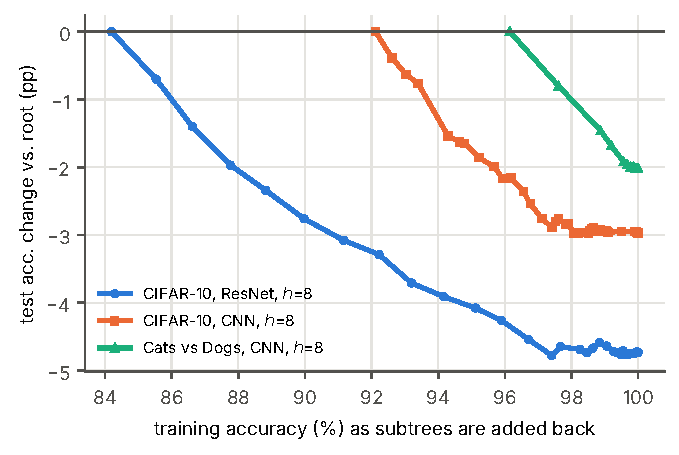
\includegraphics[width=0.55\linewidth]{prune_curve.pdf}
\caption{Cost-complexity pruning, read from right (full tree, 100\% training accuracy) to left (root
only). Each point removes one more subtree.}
\label{fig:prune}
\end{figure}

%% ---------------------------------------------------------------------------------------
\section{Interpretations and conclusions}
\label{sec:conc}

\begin{enumerate}[leftmargin=*]
\item \textbf{The tree is a constructive proof of interpolation, and a microscope on it.} The note's
  construction carries over to neural nodes almost unchanged: hinge-loss nodes, closed-form
  connection weights, and an isolation node to guarantee termination. Because every node knows which
  samples it is responsible for, the tree makes visible \emph{who} memorises \emph{what}: the root
  fits the regular structure, first-level children the atypical members of each class, deeper nodes
  individual cluttered or mislabelled-looking photographs, and -- with label noise -- most of the first-level children's positives are corrupted labels.
\item \textbf{The price of 100\% training accuracy depends on how locally one memorises.}
  Interpolation is not harmful or benign in itself. Learned correctors generalise the memorised
  points to whole regions -- deep ones literally fire on ``anything that is not a known negative'' --
  and cost up to 5 test points; isolation nodes (max-margin caps around single
  points) are a lookup table that never fires on test images and costs nothing, at the price of one
  hidden unit per memorised image. This is the tree-level version of the benign-overfitting picture
  \cite{bartlett,feldman}: memorising the long tail is harmless when it is spiky and local.
\item \textbf{Double descent is a property of the root; the tree jumps over the classical regime.}
  The peak sits exactly where the root first interpolates, with and without noise. Growing children
  reaches interpolation with far fewer parameters per node than widening, but it reaches the same
  over-parameterised error level, never the classical optimum.
\item \textbf{Features decide everything that matters.} Pixels give large trees that generalise poorly
  (60\% on Cats vs Dogs); a trunk trained on the same data hides memorisation inside the trunk;
  a set of trunks with per-node selection gives the smallest and best trees, because a node's errors
  are best separated in a feature space other than the one that produced them.
\item \textbf{Small and interpolating are at odds with good test accuracy.} The smallest
  interpolating network is the MLP at the threshold width -- the double-descent peak. Within a fixed
  tree, decision-preserving pruning removes 20--32\% of the weights for free, and cost-complexity
  pruning shows a near-linear exchange of 0.3--0.5 test points per training point.
\end{enumerate}

\paragraph{Challenges encountered.} (i) Child problems are extremely imbalanced and ``inside-out'';
without class weights the child learns ``never fire'', and linear children almost never make progress.
(ii) The connection weights of the LP are badly scaled (hundreds) -- the closed form is both exact and
better conditioned. (iii) A trunk trained on the same images inflates the root's training accuracy.
(iv) On a 2-core CPU, the trunks have to be frozen and features cached; oversubscribing the cores
slowed PyTorch down five-fold.

\section{Future directions}
\begin{itemize}[leftmargin=*]
\item \textbf{Local neural correctors.} Gate each learned corrector by an isolation cap around its
  own positives (fire only if both agree): it would keep the compactness of the network and the
  test-time locality of the lookup table.
\item \textbf{Multi-head detectors.} Replace the $K$ detectors $D_k$ by one network with $K$
  outputs and a shared hidden layer, trained jointly with the Table~II targets of all classes.
\item \textbf{Fine-tuning the trunk with the tree.} Back-propagate the corrector losses into the
  last trunk layers, so that the features themselves are reshaped to make the errors separable.
\item \textbf{Margin-based growth past interpolation.} Keep growing children for samples whose margin
  is below $\gamma>0$; by analogy with boosting~\cite{schapire} this may continue to improve test error
  after the training error is zero.
\item \textbf{Minimal-complexity nodes.} Train every node with the minimal complexity machine
  objective~\cite{mcm} or with the zero-norm~\cite{weston}, as the note suggests, to obtain the sparsest
  node that solves its sub-problem.
\end{itemize}


\bibliographystyle{plain}
\begin{thebibliography}{99}\small
\bibitem{note} Jayadeva. \emph{A tree type neural network}. Course note, 2021.
\bibitem{martinelli} G.~Martinelli, L.~P.~Ricotti, S.~Ragazzini, F.~Mascioli. A pyramidal delayed perceptron. \emph{IEEE Trans.\ Circuits and Systems}, 37(9):1176--1181, 1990.
\bibitem{weston} J.~Weston, A.~Elisseeff, B.~Sch\"olkopf, M.~Tipping. Use of the zero-norm with linear models and kernel methods. \emph{JMLR}, 3:1439--1461, 2003.
\bibitem{svmtree} A.~K.~Deb, Jayadeva, S.~Chandra. Binary classification by SVM based tree type neural networks. \emph{Proc.\ IJCNN}, 2002.
\bibitem{belkin} M.~Belkin, D.~Hsu, S.~Ma, S.~Mandal. Reconciling modern machine-learning practice and the classical bias--variance trade-off. \emph{PNAS}, 116(32), 2019.
\bibitem{nakkiran} P.~Nakkiran, G.~Kaplun, Y.~Bansal, T.~Yang, B.~Barak, I.~Sutskever. Deep double descent: where bigger models and more data hurt. \emph{ICLR}, 2020.
\bibitem{zhang} C.~Zhang, S.~Bengio, M.~Hardt, B.~Recht, O.~Vinyals. Understanding deep learning requires rethinking generalization. \emph{ICLR}, 2017.
\bibitem{feldman} V.~Feldman. Does learning require memorization? A short tale about a long tail. \emph{STOC}, 2020.
\bibitem{bartlett} P.~L.~Bartlett, P.~M.~Long, G.~Lugosi, A.~Tsigler. Benign overfitting in linear regression. \emph{PNAS}, 117(48), 2020.
\bibitem{schapire} R.~E.~Schapire, Y.~Freund, P.~Bartlett, W.~S.~Lee. Boosting the margin: a new explanation for the effectiveness of voting methods. \emph{Annals of Statistics}, 26(5), 1998.
\bibitem{simonyan} K.~Simonyan, A.~Vedaldi, A.~Zisserman. Deep inside convolutional networks: visualising image classification models and saliency maps. \emph{ICLR Workshop}, 2014.
\bibitem{lottery} J.~Frankle, M.~Carbin. The lottery ticket hypothesis: finding sparse, trainable neural networks. \emph{ICLR}, 2019.
\bibitem{mcm} Jayadeva. Learning a hyperplane classifier by minimizing an exact bound on the VC dimension. \emph{Neurocomputing}, 149:683--689, 2015.
\bibitem{timm} R.~Wightman, H.~Touvron, H.~J\'egou. ResNet strikes back: an improved training procedure in timm. \emph{arXiv:2110.00476}, 2021.
\end{thebibliography}

\appendix
\section{Code, reproduction and file map}
\label{app:code}
The private repository \url{\githuburl} contains the library, every experiment script, all result
files (JSON) behind the tables and figures, and this report's \LaTeX{} source. \texttt{run\_all.py}
lists every command in order; \texttt{README.md} documents the design.

\begin{center}\small
\begin{tabular}{@{}>{\raggedright\arraybackslash}p{0.42\linewidth}>{\raggedright\arraybackslash}p{0.54\linewidth}@{}}
\toprule
\texttt{treenn/node.py} & node networks, weighted-hinge training \eqref{eq:node}, isolation nodes\\
\texttt{treenn/tree.py} & binary tree (Table~II), closed-form and LP connection weights, OvR, corrector and gated trees\\
\texttt{treenn/trunks.py} & pixel / scratch-CNN / ResNet-18 trunks, FeatureMap\\
\texttt{treenn/receptive.py} & input-gradient receptive fields and statistics\\
\texttt{treenn/minimize.py} & decision-preserving pruning, cost-complexity subtree pruning\\
\texttt{scripts/run\_tree.py} & grow one tree; e.g.\ \texttt{--dataset catsdogs --feats cnn --model binary --h 8}\\
\texttt{scripts/run\_double\_descent.py} & width sweep, MLP vs tree\\
\texttt{scripts/receptive\_fields.py}, \texttt{analyse\_tree.py}, \texttt{run\_minimize.py} & analyses of a saved tree\\
\texttt{scripts/make\_figures.py} & all figures and tables of this report from \texttt{results/}\\
\bottomrule
\end{tabular}
\end{center}

\noindent Data: CIFAR-10 from the image-folder mirror \texttt{YoongiKim/CIFAR-10-images} (JPEG, 50k/10k),
Kaggle Cats vs Dogs from \texttt{laxmimerit/dog-cat-full-dataset} (19\,989 train / 5\,000 test as
provided by the mirror). ImageNet ResNet-18 weights: \texttt{timm} \emph{resnet18.a1\_in1k}~\cite{timm}.
Hardware: 2 CPU cores, 8\,GB RAM, no GPU.

\end{document}
